\section{Apparatus and Experiment}

The current $i$ over the capacitor is $i = C\frac{\dd v_c}{\dd t}$. Therefore,
KVL around the circuit gives 
%
\begin{equation}
    RC\frac{\dd v_c}{\dd t} + v_c = v_{\text{sig}} = A \cos{(\omega t)}
    \label{eq:de}
\end{equation} 
%
This differential equation has the transfer function \[ G(s) = \frac{1}
{RCs+1}. \] The steady-state solution of the differential equation~\eqref{eq:de}
is obtained as
%
\begin{align}
    \begin{split}
    v_c(t) &= A\abs{G(j \omega)}\cos{(\omega t + \angle G(j\omega))} \\
           &= \frac{A}{\sqrt{1+\omega^2R^2C^2}}\cos{\left(\omega t -
           \arctan{(\omega R C})\right)}
    \end{split}
    \label{eq:de_sol}
\end{align}
%
Since we do not want our signal to be attenuated by the low-pass filter, we must
choose the values of $R$ and $C$ such that $\omega R C \ll 1$ or $RC \ll
\nicefrac{1}{\omega}$. A difference of at least an order of magnitude should do
nicely.

\begin{figure}[htb]
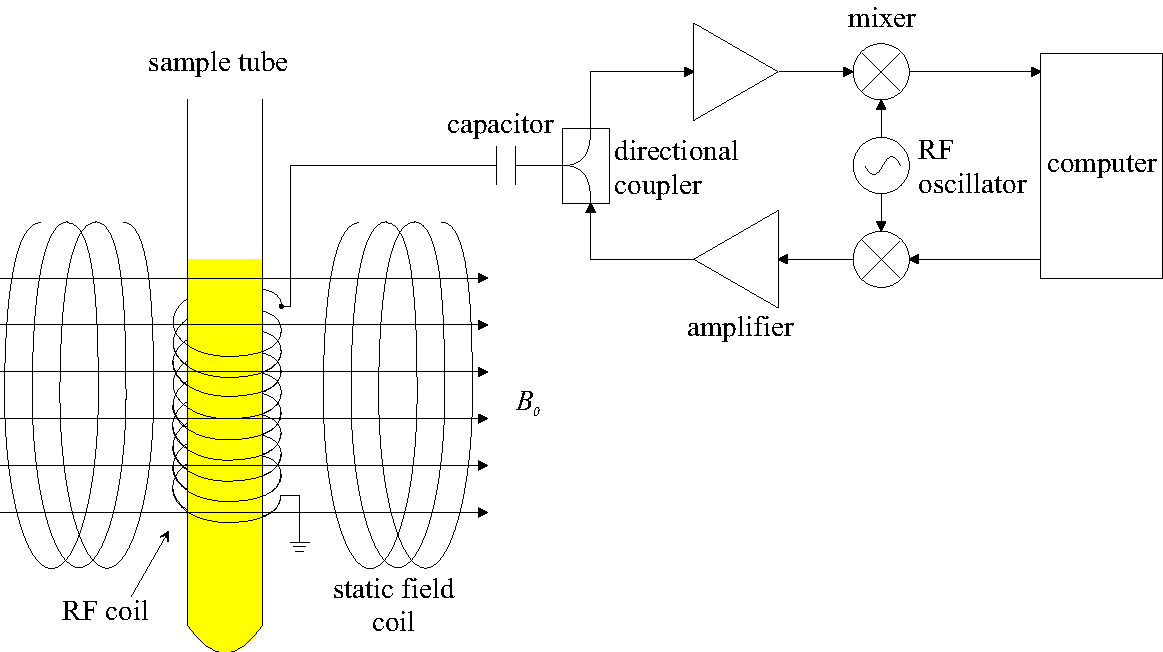
\includegraphics[width=8cm]{./figures/sample-fig1}
\caption{This is a placeholder figure until I draw the $RC$ network.}
\label{fig:RC}
\end{figure}
